\section{LIME}

LIME \cite{ribeiro2016should} is a black box interpretability method. Like all black box methods, LIME perturbates features in the input data to detect which feature is relevant for the classification. The output of LIME is a list of features which the algorithm detected as to be relevant for the classification, sorted by importance.

In the case of image classification, LIME does not modify single pixels, because this would generate too many different versions of the input.
Instead, LIME generates superpixels.

\begin{figure}[H]
\centering
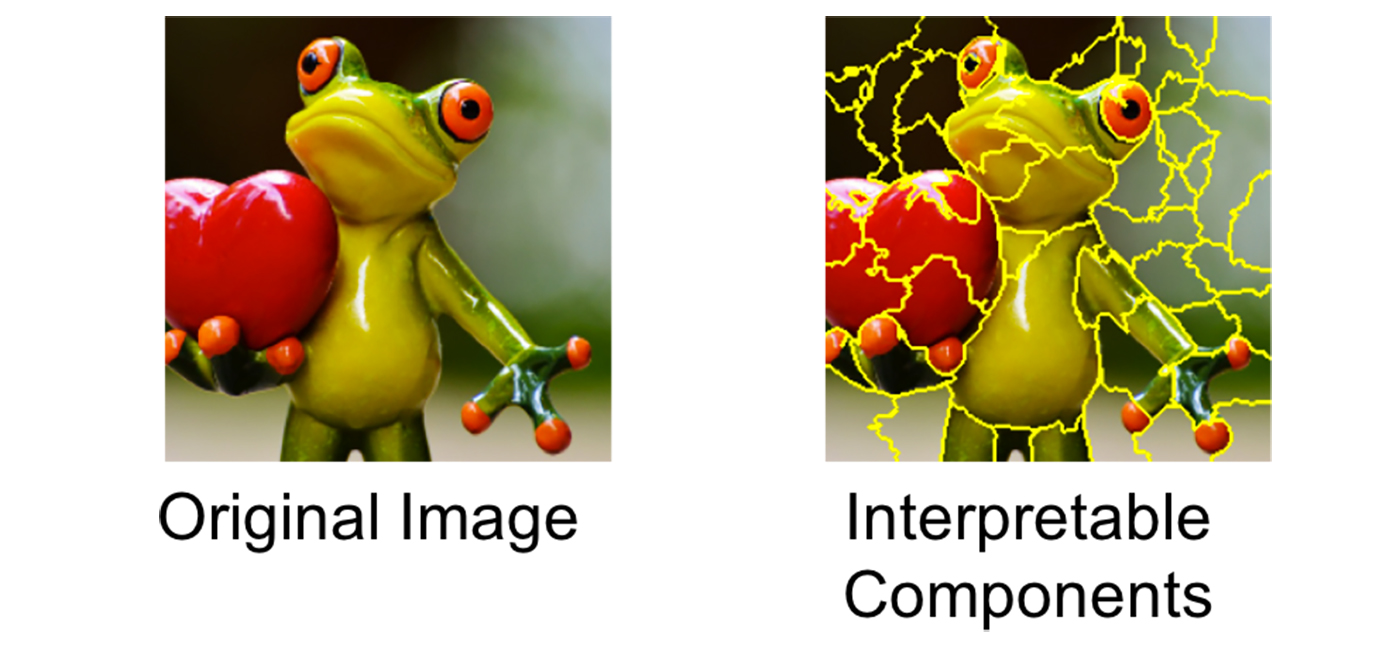
\includegraphics[width=14cm]{chapters/02_methods/images/lime.jpg}
\caption{Superpixels generated for an input image. Superpixels are the features LIME analyzes to detect if they are relevant for the classification.}
\end{figure}

Superpixels are continous regions on an image with a similar color. In the Python reference implementation, LIME uses the Quick Shift \cite{vedaldi2008quick} clustering algorithm to generate these superpixels.

In the next step, LIME generates input images by turning off randomly selected superpixels. Turning off in this case means settings the color inside the superpixel to gray.



\begin{figure}[H]
\centering
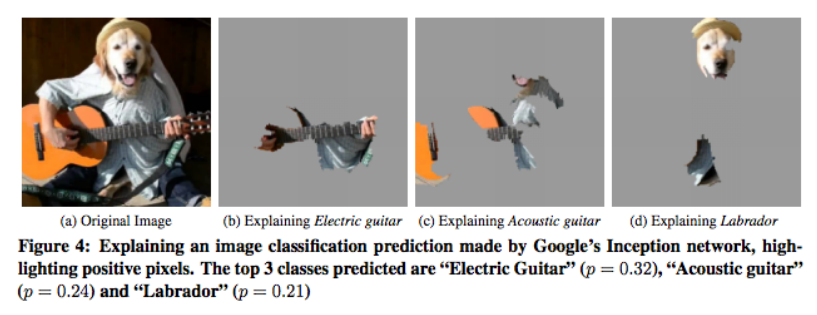
\includegraphics[width=14cm]{chapters/02_methods/images/lime.png}
\caption{Image from original LIME paper explaining three classes.}
\end{figure}
